\documentclass[../notes.tex]{subfiles}

\pagestyle{main}
\renewcommand{\chaptermark}[1]{\markboth{\chaptername\ \thechapter\ (#1)}{}}
\setcounter{chapter}{12}

\begin{document}




\chapter{Dynamical Systems and Chaos}
\section{Introduction to Dynamical Systems; Phase Portraits}
\begin{itemize}
    \item \marginnote{11/27:}\textbf{Dyanmical system}: A system of first-order ODEs.
    \item Example: Flows on a line.
    \begin{figure}[h!]
        \centering
        \begin{tikzpicture}
            \footnotesize
            \draw [
                -stealth,
                decoration={
                    markings,
                    mark=at position 0.15 with \arrow{<},
                    mark=at position 0.40 with \arrow{>},
                    mark=at position 0.65 with \arrow{>},
                    mark=at position 0.87 with \arrow{<}
                },
                postaction=decorate
            ] (-1,0) -- (1,0) node[right]{$x$};
            \draw [-stealth] (0,-0.5) -- (0,1.5) node[above]{$f(x)=\dot{x}$};
    
            \draw [grx,thick,<->] plot[domain=-0.6:0.6] (\x,{1-4*\x*\x});
    
            \filldraw [fill=white] (-0.5,0) circle (1pt);
            \filldraw              (0.5,0)  circle (1pt);
        \end{tikzpicture}
        \caption{Dynamical flows on a line.}
        \label{fig:flowsLine}
    \end{figure}
    \begin{itemize}
        \item Consider
        \begin{equation*}
            \dot{x} = -x^2+4
        \end{equation*}
        \item Graph $f(x)=\dot{x}$, as above.
        \item When the graph is negative, a particle on the line heads to the left; when it is positive, the particle heads to the right. We indicate this with arrows.
        \item Then we indicate \textbf{fixed points} with circles, \textbf{unstable} ones with unfilled circles and \textbf{stable} ones with filled circles.
        \item How do we determine fixed points and stability mathematically?
        \item Fixed points: Solving $\dot{x}=0$ yields $x^*=\pm 2$ as fixed points.
        \item Stability: Consider a point a small distance away from $x^*$ at $x=x^*+\xi$.
        \begin{itemize}
            \item Approximate $\dot{x}$ near $x^*$ via
            \begin{equation*}
                \dot{x} = f(x) = f(x^*+\xi) \approx f(x^*)+\eval{\pdv{f}{x}}_{x^*}\xi+O(\xi^2)
            \end{equation*}
            \item Then since $f(x^*)=0$ and we neglect $O(\xi^2)$ for small $\xi$, we have that
            \begin{equation*}
                \dot{x} = \dot{\xi} = \eval{\pdv{f}{x}}_{x^*}\xi
            \end{equation*}
            \item Looking at Figure \ref{fig:flowsLine}, we can see that the fixed point is stable if $\eval{\pdv*{f}{x}}_{x^*}\xi<0$ and unstable if $\eval{\pdv*{f}{x}}_{x^*}\xi>0$.
        \end{itemize}
    \end{itemize}
    \item \textbf{Fixed point}: A point at which $\dot{x}=0$.
    \item \textbf{Unstable} (fixed point): A fixed point with the flow heading away from it.
    \item\textbf{Stable} (fixed point): A fixed point with the flow heading toward it.
    \item Let's promote ourselves up a dimension to the 2D phase plane.
    \item Example: Pendulum.
    \begin{figure}[h!]
        \centering
        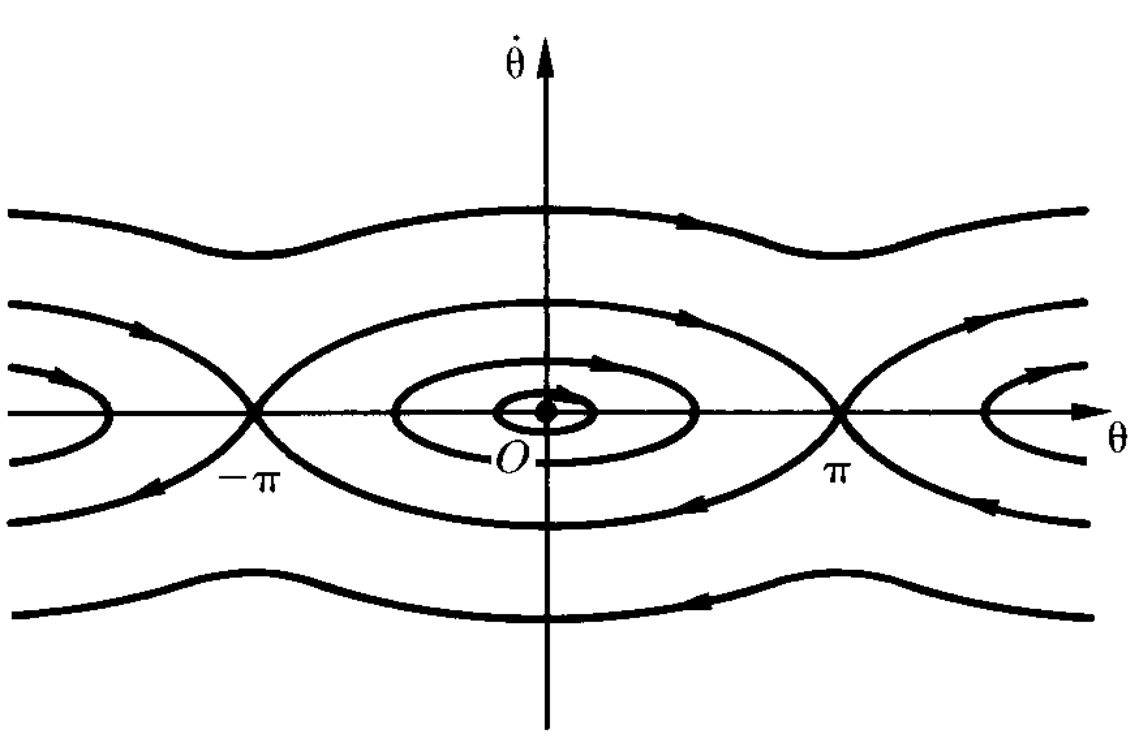
\includegraphics[width=0.4\linewidth]{../ExtFiles/flowsPendulum.png}
        \caption{Dynamical flows of a pendulum.}
        \label{fig:flowsPendulum}
    \end{figure}
    \begin{itemize}
        \item Recall that the Hamiltonian for such a system is
        \begin{equation*}
            H = \frac{p_\theta^2}{2m\ell^2}-mg\ell\cos\theta
        \end{equation*}
        \item Thus, Hamilton's equations are
        \begin{align*}
            -\dot{p}_\theta &= \pdv{H}{\theta} = mg\ell\sin\theta&
            \dot{\theta} &= \pdv{H}{p_\theta} = \frac{p_\theta}{m\ell^2}
        \end{align*}
        \item This gives us a system of first-order ODEs.
        \item Fixed points: $\dot{\theta}=0$ implies $p_\theta=0$, implies $\dot{p}_\theta=0$, implies $\sin\theta=0$ implies $\theta=0,\pm\pi,\dots$.
        \item We may now draw a \textbf{phase portrait}.
        \item We get circles corresponding to the switch between momentum and potential energy.
        \item At the fixed points, we have a special \textbf{separatrix}; the particle takes an infinite amount of time to get to the fixed point with unstable equilibrium.
        \item Then the paths at the top and bottom are other trajectories corresponding to swinging all the way around in one direction or another.
        \item It is traditional to call these paths \emph{trajectories}, even though they are not physical trajectories $x(t)$.
    \end{itemize}
    \item \textbf{Phase portrait}: A plot that gives the paths of particles at all times.
    \begin{itemize}
        \item What you gain from a phase portrait is all of the paths, but what you lose is all of the dynamical information (i.e., you have no idea how fast anything is going).
    \end{itemize}
    \item Linear stability in 2D.
    \begin{itemize}
        \item In general, we have a system of two first-order ODEs as follows.
        \begin{equation*}
            \begin{cases}
                \dot{x} = f(x,y)\\
                \dot{y} = g(x,y)
            \end{cases}
        \end{equation*}
        \item Let $(x^*,y^*)$ be a fixed point.
        \item Then, Taylor expanding, we get
        \begin{align*}
            \dot{x} &= f(x^*+\xi,y^*+\eta) \approx f(x^*,y^*)+\eval{\pdv{f}{x}}_{x^*,y^*}\xi+\eval{\pdv{f}{y}}_{x^*,y^*}\eta+O(\xi^2,\eta^2)\\
            \dot{y} &= g(x^*+\xi,y^*+\eta) \approx g(x^*,y^*)+\eval{\pdv{g}{x}}_{x^*,y^*}\xi+\eval{\pdv{g}{y}}_{x^*,y^*}\eta+O(\xi^2,\eta^2)
        \end{align*}
        \item From here, we obtain a matrix of coefficients called the \textbf{Jacobian matrix}, $J$, as follows.
        \begin{equation*}
            \begin{pmatrix}
                \dot{x}\\
                \dot{y}\\
            \end{pmatrix}
            =
            \begin{pmatrix}
                \dot{\xi}\\
                \dot{\eta}\\
            \end{pmatrix}
            =
            \begin{pNiceMatrix}
                \pdv{f}{x} & \pdv{f}{y}\\
                \pdv{g}{x} & \pdv{g}{y}\\
            \end{pNiceMatrix}
            \begin{pmatrix}
                \xi\\
                \eta\\
            \end{pmatrix}
        \end{equation*}
        \begin{itemize}
            \item The directions of exponential growth and decay occur in the eigendirections of the Jacobian matrix!
        \end{itemize}
        \item Indeed, in these 2D systems, we can classify the fixed point based on the eigenvalues of $J$.
        \item Solve for the eigenvalues using the following formula.
        \begin{equation*}
            \lambda_{1,2} = \frac{1}{2}\left[ \tr(J)\pm\sqrt{\tr(J)^2-4\det(J)} \right]
        \end{equation*}
        \item For stability, we need the real parts of both eigenvalues to be less than zero.
    \end{itemize}
    \item There are three important classifications of such systems.
    \begin{figure}[h!]
        \centering
        \begin{subfigure}[b]{0.24\linewidth}
            \centering
            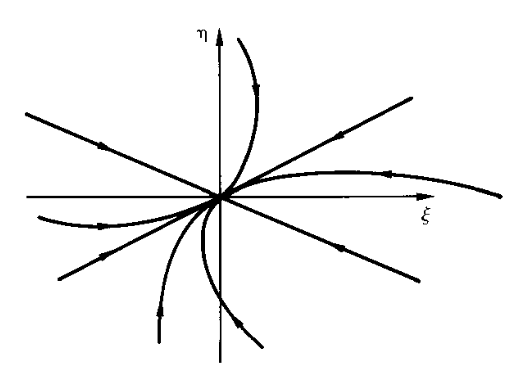
\includegraphics[width=0.95\linewidth]{../ExtFiles/flows2Da.png}
            \caption{Node.}
            \label{fig:flows2Da}
        \end{subfigure}
        \begin{subfigure}[b]{0.24\linewidth}
            \centering
            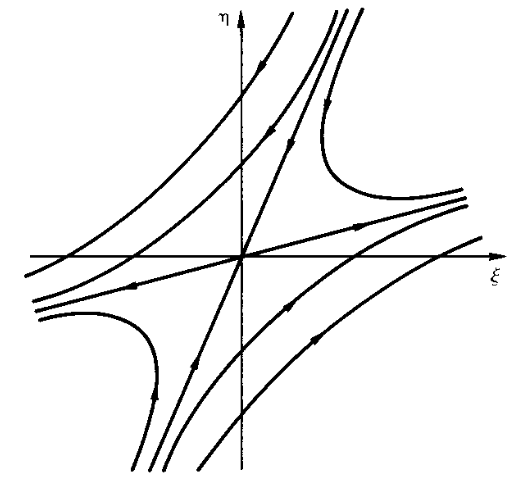
\includegraphics[width=0.95\linewidth]{../ExtFiles/flows2Db.png}
            \caption{Saddle.}
            \label{fig:flows2Db}
        \end{subfigure}
        \begin{subfigure}[b]{0.24\linewidth}
            \centering
            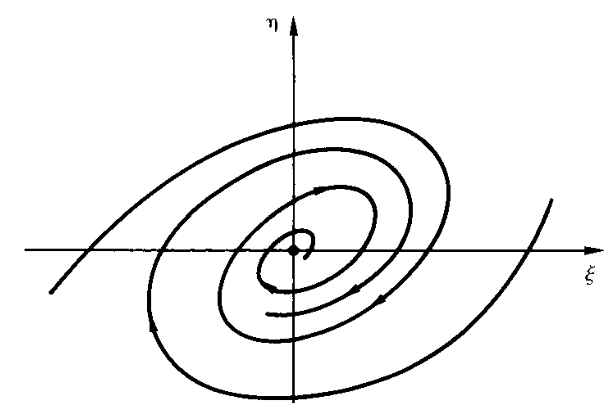
\includegraphics[width=0.95\linewidth]{../ExtFiles/flows2Dc.png}
            \caption{Spiral.}
            \label{fig:flows2Dc}
        \end{subfigure}
        \begin{subfigure}[b]{0.24\linewidth}
            \centering
            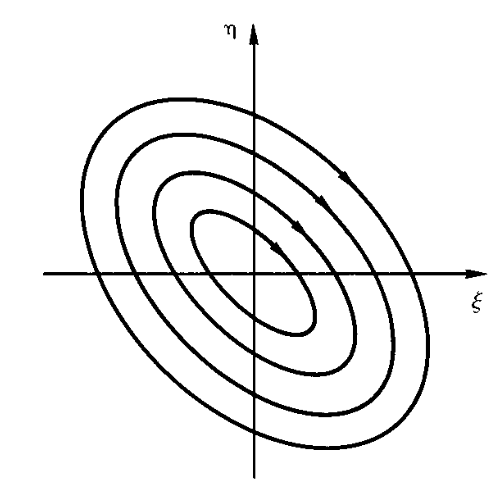
\includegraphics[width=0.95\linewidth]{../ExtFiles/flows2Dd.png}
            \caption{Center.}
            \label{fig:flows2Dd}
        \end{subfigure}
        \caption{Dynamical flows of a 2D system.}
        \label{fig:flows2D}
    \end{figure}
    \begin{enumerate}
        \item \textbf{Nodes} happen when both $\lambda_1,\lambda_2$ are real and both are positive \emph{or} both are negative.
        \begin{itemize}
            \item Everything falls into the fixed point in the case $\lambda_1,\lambda_2<0$; some things directly (along eigendirections) and other things along curved paths.
            \item Alternatively, if $\lambda_1,\lambda_2>0$, then everything gets blown away.
        \end{itemize}
        \item If one is greater than zero and one is less than zero, we get a \textbf{saddle} point.
        \item If there are some imaginary parts, we get circulation and spiraling. From the eigenvalue formula, we can see that $\lambda_1,\lambda_2=a\pm bi$ are complex conjugates.
        \begin{itemize}
            \item If real parts are negative, we spiral inwards; if positive, we spiral outwards.
            \item There's also the concept of a \textbf{center}; when $\lambda_1,\lambda_2$ are purely imaginary, we get pure circulation where things choose their orbit and stay on it. This is also \emph{stable}, even though things don't fall into the node.
        \end{itemize}
    \end{enumerate}
    \item A handy picture to help us classify any fixed point we want in two dimensions.
    \begin{figure}[h!]
        \centering
        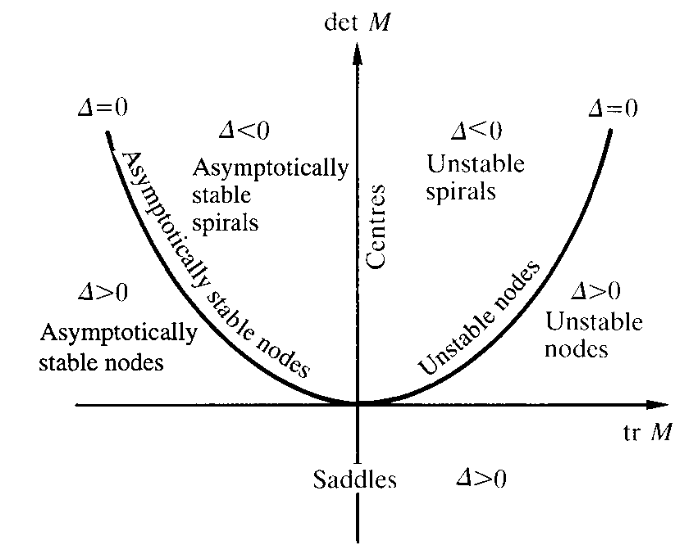
\includegraphics[width=0.4\linewidth]{../ExtFiles/fixedPoints2D.png}
        \caption{Classifying fixed points of a 2D system.}
        \label{fig:fixedPoints2D}
    \end{figure}
    \begin{itemize}
        \item If we look at systems defined in terms of their trace and determinant, there is a sideways parabola defined by the discriminant of the eigenvalue formula, i.e., via $\tr(J)^2-4\det(J)=0$.
        \item Various paths live in different parts of the map.
    \end{itemize}
\end{itemize}



\section{Bifurcations; Order and Chaos in Hamiltonian Systems}
\begin{itemize}
    \item \marginnote{11/29:}Outline.
    \begin{itemize}
        \item Bifurcations.
        \item Integrability and chaos.
    \end{itemize}
    \item Today.
    \begin{itemize}
        \item Ambitous plan:
        \item Dynamical systems and phase portraits.
        \item What bifurcations are and why they're interesting.
        \item When a system is ordered or chaotic.
    \end{itemize}
    \item Recap.
    \begin{itemize}
        \item Definition of a \textbf{dyanmical system}.
        \item Recall that Hamilton's equations can help us describe motion in a phase plane through a phase portrait.
        \item Essentially, the system of equations defines a vector field $(\dot{q},\dot{p})$ at each point $(q,p)$ in the plane. Moreover, trajectories run tangent to vectors.
        \item We also saw last time that near a fixed point, for a 2D system $\dot{x}=f(x,y)$ and $\dot{y}=g(x,y)$ such that there exists a point $(x^*,y^*)$ such that $f(x^*,y^*)=g(x^*,y^*)=0$. Then if we perturb a bit away from this point, our perturbation is given by the Jacobian matrix formula.
        \item It follows that we can classify fixed points based on the eigenvalues of the Jacobian, which are given by $\lambda_{1,2}=(\tr(J)\pm\sqrt{\tr(J)^2-4\det(J)})/2$.
        \item Recall Figure \ref{fig:fixedPoints2D}.
    \end{itemize}
    \item Why do the eigenvalues of the Jacobian matrix control the fixed point?
    \begin{itemize}
        \item Let
        \begin{equation*}
            \vec{\nu} =
            \begin{pmatrix}
                \xi\\
                \eta\\
            \end{pmatrix}
        \end{equation*}
        so that
        \begin{equation*}
            \dot{\vec{\nu}} = J\vec{\nu}
        \end{equation*}
        \item Diagonalize $J$ to $J=R^{-1}DR$. Then
        \begin{align*}
            \dot{\vec{\nu}} &= R^{-1}DR\vec{\nu}\\
            R\dot{\vec{\nu}} &= DR\vec{\nu}\\
            \dv{t}\underbrace{(R\vec{\nu})}_\mu &= D\underbrace{(R\vec{\nu})}_\mu\\
            \dot{\mu} &= D\mu
        \end{align*}
        uncouples into
        \begin{align*}
            \dot{\mu}_1 &= \lambda_1\mu_1&
                \dot{\mu}_2 &= \lambda_2\mu_2\\
            \mu_1 &= A\e[\lambda_1t]&
                \mu_2 &= A\e[\lambda_2t]
        \end{align*}
    \end{itemize}
    \item Now let's talk about classifying fixed points in the context of conservative Hamiltonian systems with one degree of freedom.
    \begin{itemize}
        \item In this case, we have 
        \begin{align*}
            p &= m\dot{x}&
            H &= \frac{p^2}{2m}+V(x)
        \end{align*}
        \item Hamilton's equations then give us
        \begin{align*}
            \dot{x} &= \pdv{H}{p} = \frac{p}{m}&
            \dot{p} &= -\pdv{H}{x} = -\dv{V}{x}
        \end{align*}
        \item Now define
        \begin{align*}
            f(x,p) &= \dot{x} = \frac{p}{m}&
            g(x,p) &= \dot{p} = -\dv{V}{x}
        \end{align*}
        \item Thus, the Jacobian matrix is
        \begin{equation*}
            J =
            \begin{pNiceMatrix}
                0 & \frac{1}{m}\\
                -V''(x) & 0\\
            \end{pNiceMatrix}
        \end{equation*}
        with
        \begin{align*}
            \tr(J) &= 0&
            \det(J) &= \frac{V''(x)}{m}
        \end{align*}
        \item Thus, according to Figure \ref{fig:fixedPoints2D}, if $V''(x)>0$, we get a center, and if $V''(x)<0$, we get a saddle.
        \item More specifically, if $V''(x)>0$, then from the eigenvalues formula,
        \begin{equation*}
            \lambda_{1,2} = i\omega
        \end{equation*}
        where
        \begin{equation*}
            \omega = \sqrt{\frac{V''(x)}{m}}
        \end{equation*}
        \item Recall the pendulum picture, Figure \ref{fig:flowsPendulum}.
        \item In this conservative system, we have a fixed energy $E=p^2/2m+V(x)$. All of the trajectories in Figure \ref{fig:flowsPendulum} are level sets of $E$. So we pick our energy, and the $p(x)=\pm\sqrt{2m(E-V(x))}$, so you can plug in your favorite $V$, and you will get $p$.
    \end{itemize}
    \item Now let's talk about \textbf{bifurcations}.
    \item One of the nice things that this dynamical systems picture gives us is an idea of when a system is going to \emph{really} change.
    \item \textbf{Bifurcation}: A number or type of fixed point changes.
    \item Prototypical type of bifurcation: A \textbf{sattle-node} bifurcation.
    \begin{figure}[h!]
        \centering
        \begin{subfigure}[b]{0.2\linewidth}
            \centering
            \begin{tikzpicture}
                \footnotesize
                \draw [
                    decoration={
                        markings,
                        mark=at position 0.23 with \arrow{>},
                        mark=at position 0.43 with \arrow{<},
                        mark=at position 0.6 with \arrow{<},
                        mark=at position 0.8 with \arrow{>}
                    },
                    postaction=decorate
                ] (-1,0) -- (1,0) node[right]{$x$};
                \draw (0,-1) -- (0,1) node[above]{$\dot{x}$};
        
                \draw [grx,thick] plot[domain=-0.6:0.6] (\x,{4*\x*\x-0.5});
        
                \filldraw              (-0.354,0) circle (1pt);
                \filldraw [fill=white] (0.354,0)  circle (1pt);
            \end{tikzpicture}
            \caption{$r<0$.}
            \label{fig:bifurSaddleNodea}
        \end{subfigure}
        \begin{subfigure}[b]{0.2\linewidth}
            \centering
            \begin{tikzpicture}
                \footnotesize
                \draw [
                    decoration={
                        markings,
                        mark=at position 0.25 with \arrow{>},
                        mark=at position 0.75 with \arrow{>}
                    },
                    postaction=decorate
                ] (-1,0) -- (1,0) node[right]{$x$};
                \draw (0,-1) -- (0,1) node[above]{$\dot{x}$};
        
                \draw [grx,thick] plot[domain=-0.5:0.5] (\x,{4*\x*\x});
        
                \filldraw [fill=white] (-0,0) circle (1pt);
                \fill (0,1pt) arc[start angle=90,end angle=270,radius=1pt];
            \end{tikzpicture}
            \caption{$r=0$.}
            \label{fig:bifurSaddleNodeb}
        \end{subfigure}
        \begin{subfigure}[b]{0.2\linewidth}
            \centering
            \begin{tikzpicture}
                \footnotesize
                \draw [
                    decoration={
                        markings,
                        mark=at position 0.25 with \arrow{>},
                        mark=at position 0.75 with \arrow{>}
                    },
                    postaction=decorate
                ] (-1,0) -- (1,0) node[right]{$x$};
                \draw (0,-1) -- (0,1) node[above]{$\dot{x}$};
        
                \draw [grx,thick] plot[domain=-0.35:0.35] (\x,{4*\x*\x+0.5});
            \end{tikzpicture}
            \caption{$r>0$.}
            \label{fig:bifurSaddleNodec}
        \end{subfigure}\\[1em]
        \begin{subfigure}[b]{0.3\linewidth}
            \centering
            \begin{tikzpicture}
                \footnotesize
                \draw (-2,0) -- (2,0) node[right]{$r$};
                \draw (0,-1) -- (0,1) node[above]{$x$};
        
                \draw [orx,thick,densely dashed] plot[domain=0:0.7] ({-4*\x*\x},{\x});
                \draw [orx,thick] plot[domain=-0.7:0] ({-4*\x*\x},{\x});
    
                \node at (-1,-0.7) {stable};
                \node at (-1,0.75) {unstable};
            \end{tikzpicture}
            \caption{Bifurcation diagram.}
            \label{fig:bifurSaddleNoded}
        \end{subfigure}
        \caption{Saddle-node bifurcation.}
        \label{fig:bifurSaddleNode}
    \end{figure}
    \begin{itemize}
        \item One-dimensional example: Consider $\dot{x}=r+x^2$.
        \item As $r$ varies from negative to zero to postive, we get the Figure \ref{fig:bifurSaddleNodea}-\ref{fig:bifurSaddleNodec}. First two fixed points, then one, then none.
        \item A \textbf{bifurcation diagram} plots $r$ vs. the $x$-position of the fixed points, stable ones with solid lines and unstable ones with dotted lines. See Figure \ref{fig:bifurSaddleNoded}.
    \end{itemize}
    \item There's a lovely taxonomy of many types of bifurcations. We don't have time to go into them, but here's another one that comes up a lot in physics (we'll talk about it further in discussion section).
    \item The \textbf{pitchfork bifurcation}.
    \begin{figure}[h!]
        \centering
        \begin{subfigure}[b]{0.2\linewidth}
            \centering
            \begin{tikzpicture}
                \draw [grx,thick] plot[domain=-1:1,smooth] (\x,{2/2*(\x)^2+1*(\x)^4});
            \end{tikzpicture}
            \caption{$S>0$.}
            \label{fig:bifurPitchforka}
        \end{subfigure}
        \begin{subfigure}[b]{0.2\linewidth}
            \centering
            \begin{tikzpicture}
                \draw [grx,thick] plot[domain=-1.39:1.39,smooth] (\x,{-2/2*(\x)^2+1*(\x)^4});
            \end{tikzpicture}
            \caption{$S<0$.}
            \label{fig:bifurPitchforkb}
        \end{subfigure}\\[1em]
        \begin{subfigure}[b]{0.3\linewidth}
            \centering
            \begin{tikzpicture}
                \footnotesize
                \draw (-2,0) -- (2,0) node[right]{$r$};
                \draw (0,-1) -- (0,1) node[above]{$x$};
        
                \draw [orx,thick] plot[domain=-0.7:0.7] ({-4*\x*\x},{\x});
                \draw [orx,thick,densely dashed] (-2,0) -- (0,0);
                \draw [orx,thick] (0,0) -- (2,0);
            \end{tikzpicture}
            \caption{Bifurcation diagram.}
            \label{fig:bifurPitchforkc}
        \end{subfigure}
        \caption{Pitchfork bifurcation.}
        \label{fig:bifurPitchfork}
    \end{figure}
    \begin{itemize}
        \item Consider a potential well of the form
        \begin{equation*}
            V(x) = \frac{S}{2}x^2+ux^4
        \end{equation*}
        \item There are two important cases here.
        \begin{enumerate}
            \item If $S>0$, we get a single well (see Figure \ref{fig:bifurPitchforka}).
            \item If $S<0$, then the well divides into two (see Figure \ref{fig:bifruPitchforkb}).
        \end{enumerate}
        \item The particle always wants to slide toward the minimum potential energy, so in the first case, we have on stable branch, and in the second case, we develop three stable branches and one unstable branch. See Figure \ref{fig:bifurPitchforkc}.
    \end{itemize}
    \item We now return to rigid-body rotation.
    \begin{figure}[h!]
        \centering
        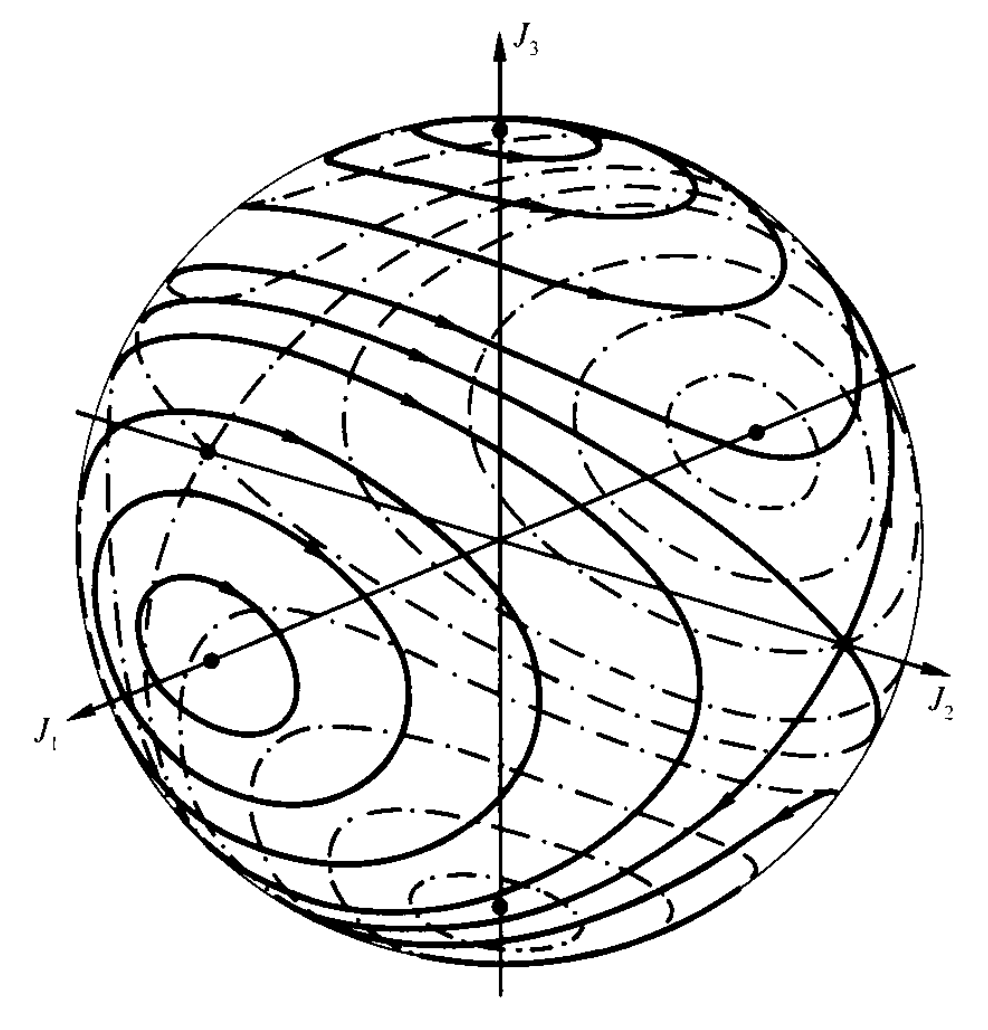
\includegraphics[width=0.4\linewidth]{../ExtFiles/flowsRigid.png}
        \caption{Dynamical flows of a rotating rigid body.}
        \label{fig:flowsRigid}
    \end{figure}
    \begin{itemize}
        \item We'll look at this problem more in the last problem of PSet 7.
        \item Recall the following equation for a rigid body with no external torque.
        \begin{equation*}
            \underbrace{I_1\dot{\omega}_1}_{\dot{J}_1}+(I_3-I_2)\omega_2\omega_3 = 0
        \end{equation*}
        \item This equation can be rewritten in the form
        \begin{align*}
            \dot{J}_1-\frac{I_2-I_3}{I_2I_3}J_2J_3 &= 0\\
            \dot{J}_2-\frac{I_1-I_3}{I_1I_3}J_1J_3 &= 0\\
            \dot{J}_3-\frac{I_2-I_1}{I_1I_2}J_2J_1 &= 0
        \end{align*}
        \item We have the conservation laws
        \begin{align*}
            J_1^2+J_2^2+J_3^2 &= J&
            \frac{J_1^2}{I_1}+\frac{J_2^2}{I_2}+\frac{J_3^2}{I_3} &= 2T
        \end{align*}
        \item Thus the fixed points arise as points on a unit sphere where one axis has unit value and the other two have none. These represent rotation about each fixed axis.
        \item As we'd expect from the tennis raquet theorem, the largest ones are stable, and the remaining intermediate axis has saddle points which defines separatrices that interpolate between the other centers.
        \item Fixed points: $J_3^2=J^2$, $J_1,J_2=0$.
    \end{itemize}
    \item We now try to understand the possible types of long-term behavior in a system.
    \item Here are the options.
    \begin{enumerate}
        \item Flow to a fixed point (this is an equilibrium situation, common especially in system with dissipation).
        \item Systems can oscillate forever (two common cases are centers, which often arise in Hamiltonian systems with energy conservation [planets, pendulums, etc.] and limit cycles of nonlinear systems).
        \item Strange attractor (leads to \textbf{chaos}).
    \end{enumerate}
    \item The most canonical set of equations that display chaos (though many systems due this in certain parameter regimes) is the \textbf{Lorentz system}, an extremely simplified model of fluid convection between parallel plates at different temperatures.
    \item \textbf{Lorentz system}:
    \begin{align*}
        \dot{x} &= \sigma(y-x)&
        \dot{y} &= \rho x-y-xz&
        \dot{z} &= -\beta z+xy
    \end{align*}
    \begin{itemize}
        \item We watched a \href{https://youtu.be/q3kNHomvU0k?t=26}{video} in class.
        \item We get attraction to a certain manifold.
        \item There's a picture in the textbook.
    \end{itemize}
    \item Characteristics of chaotic systems.
    \begin{enumerate}
        \item Aperiodic long-term behavior in a deterministic system.
        \item Sensitive dependence on initial conditions.
        \begin{itemize}
            \item This means that if you have two different trajectories in the phase plane that are separated by distance $d_0$ at time $t=0$, then the separation $d$ at time $t$ is exponentially dependent on time via $d=d_0\e[\lambda t]$ where $\lambda$ is a \textbf{Lyapunov exponent}.
        \end{itemize}
    \end{enumerate}
    \item Hamiltonian systems.
    \begin{itemize}
        \item $n$ generalized coordinates.
        \item Phase space: $2n$.
        \item Number of conserved quantities: $k$.
        \item Dimension of the restricted space is $M=2n-k$.
        \item If $k\geq n$, the system is \textbf{integrable} and there is no chaos, whereas if $k<n$, then there will be chaos in \emph{some} parameter.
        \item The damped, forced pendulum; top with external torques; etc. fall in this regime, so this kind of motion is not hard to find.
    \end{itemize}
\end{itemize}



\section{Final Exam Review}
\begin{itemize}
    \item \marginnote{12/1:}Announcements.
    \begin{itemize}
        \item Thanks for a great quarter!
        \item Fill out course evals.
    \end{itemize}
    \item Our problem.
    \begin{itemize}
        \item We have $N$ particles with initial positions $\vec{x}_1(0),\dots,\vec{x}_N(0)$ in 3D space and initial momenta $\vec{p}_1(0),\dots,\vec{p}_N(0)$.
        \item We want to know what they will do, i.e., what is $\vec{x}_i(t)$ for all $i=1,\dots,N$ and $t>0$.
    \end{itemize}
    \item 2-body systems (Chapter 7).
    \begin{itemize}
        \item The center of mass $\vec{R}$ and relative position $\vec{r}$ are given by
        \begin{align*}
            \vec{R} &= \frac{m_1\vec{r}_1+m_2\vec{r}_2}{m_1+m_2}&
            \vec{r} &= \vec{r}_1-\vec{r}_2
        \end{align*}
        \item We also define the total mass $M$ and reduced mass $\mu$ by
        \begin{align*}
            M &= m_1+m_2&
            \mu &= \frac{m_1m_2}{m_1+m_2}
        \end{align*}
        \item Under the constant force of gravity\dots
        \begin{itemize}
            \item The Lagrangian for the system is
            \begin{equation*}
                L = \frac{1}{2}M\dot{\vec{R}}^2+M\vec{g}\cdot\vec{R}+\frac{1}{2}\mu\dot{\vec{r}}^2-V_\text{int}(\vec{r})
            \end{equation*}
            \item The EOMs separate into
            \begin{align*}
                M\ddot{\vec{R}} &= M\vec{g}\\
                \mu\ddot{\vec{r}} &= \vec{F}_{12}
            \end{align*}
            where the second equation above is that of a one-body problem.
            \item We then solve for $\vec{r},\vec{R}$ and use these to find $\vec{r}_1,\vec{r}_2$ via
            \begin{align*}
                r_1 &= \vec{R}+\frac{m_2}{M}\vec{r}\\
                r_2 &= \vec{R}-\frac{m_1}{M}\vec{r}
            \end{align*}
        \end{itemize}
        \item It is often useful to do this in the center of mass frame (*).
        \begin{itemize}
            \item We convert into this frame with
            \begin{align*}
                \vec{r}_1{}^* &= +\frac{m_2}{M}\vec{r}\\
                \vec{r}_2{}^* &= -\frac{m_1}{M}\vec{r}
            \end{align*}
            \item In the CM frame, we have the following laws.
            \begin{align*}
                P^* &= 0&
                J^* &= \mu\vec{r}\times\dot{\vec{r}}&
                T^* &= \frac{1}{2}\mu\dot{\vec{r}}{\,}^2
            \end{align*}
            \item In the lab frame, we have the following laws.
            \begin{align*}
                \vec{P} &= M\vec{R}&
                \vec{J} &= M\vec{R}\times\dot{\vec{R}}+J^*&
                T &= \frac{1}{2}M\dot{\vec{R}}{\,}^2+T^*
            \end{align*}
        \end{itemize}
    \end{itemize}
    \item Moving onto many-body systems (Chapter 8).
    \begin{itemize}
        \item We generalize the center of mass to
        \begin{equation*}
            \vec{R} = \frac{1}{M}\sum_\alpha m_\alpha\vec{r}_\alpha
        \end{equation*}
        where $M=\sum_\alpha m_\alpha$.
        \item Within the CM frame (*),
        \begin{align*}
            \vec{r}_\alpha &= \vec{R}+\vec{r}_\alpha{}^*&
            \vec{J}{\,}^* &= \sum_\alpha m_\alpha\vec{r}_\alpha{}^*\times\dot{\vec{r}}_\alpha{}^*&
            T^* &= \sum_\alpha\frac{1}{2}m_\alpha\dot{\vec{r}}_\alpha{}^2
        \end{align*}
        \item Within the lab frame,
        \begin{align*}
            \vec{P} &= M\dot{\vec{R}}&
            \vec{J} &= M\vec{R}\times\dot{\vec{R}}+J^*&
            T &= \frac{1}{2}M\dot{\vec{R}}{\,}^2+T^*
        \end{align*}
        \item For no force or constant force (like gravity), the Hamiltonian and Lagrangian separate into CM and rest of system.
        \item Such problems are hard to solve in general, so we quickly specified to rigid bodies.
    \end{itemize}
    \item Rigid bodies (Chapter 9 + a bit of 10).
    \begin{itemize}
        \item No changes in internal potential energy.
        \item We define the angular momentum of the whole system as
        \begin{equation*}
            \vec{J} = \overleftrightarrow{I}\vec{\omega}
        \end{equation*}
        where $\overleftrightarrow{I}$ is the moment of inertia tensor and $\vec{\omega}$ is the instantaneous angular velocity.
        \item There is a special set of coordinates here called the principal axes. In the basis of the principal axes $\hat{e}_1,\hat{e}_2,\hat{e}_3$, the moment of inertia tensor is diagonal, i.e.,
        \begin{equation*}
            \overleftrightarrow{I} =
            \begin{bmatrix}
                I_1 & 0 & 0\\
                0 & I_2 & 0\\
                0 & 0 & I_3\\
            \end{bmatrix}
        \end{equation*}
        where
        \begin{equation*}
            I_1 = \int\dd{V}\rho_m(y^2+z^2)
        \end{equation*}
        for $\rho_m$ the density, and similarly for $I_2,I_3$.
        \item The products of inertia vanish for these axes; we can use this as a check.
        \item How do we find a moment of inertia?
        \begin{itemize}
            \item Use the parallel axis theorem, which tells us that
            \begin{equation*}
                I_1 = M(X^2+Y^2)+I_1^*
            \end{equation*}
            where $I_1^*$ is $I_1$ with the origin at the center of mass and $X,Y$ are center of mass coordinates.
            \item Have Routh's Rules in our mind or in our note's sheet! These are the factors for cylindrical, ellipsoidal, parallelepiped, etc. symmetry. Very important!
        \end{itemize}
        \item In the principal axis basis,
        \begin{equation*}
            \vec{J} = I_1\omega_1\hat{e}_1+I_2\omega_2\hat{e}_2+I_3\omega_3\hat{e}_3
        \end{equation*}
        \item The equations of motion for a rigid body:
        \begin{align*}
            \dot{\vec{J}} &= \sum\vec{r}\times\vec{F}&
            \dot{\vec{P}} &= M\ddot{\vec{R}} = \sum\vec{F}
        \end{align*}
        \begin{itemize}
            \item These equations of motion can help us answer questions such as, "why does a spinning top not fall over?"
            \item Here, the EOMs are $\vec{J}=I_3\omega\hat{e}_3$ and $\vec{F}=-Mg\khat$.
            \item Essentially, we have a torque, which is a change in $\vec{J}$ in the $-\hat{e}_3\times\khat$ direction.
            \item This causes $\vec{\omega}$ to rotate, leading to the phenomenon of precession.
            \item What balances gravity is $M\ddot{\vec{R}}=\sum\vec{F}=\vec{F}_\text{pivot}+\vec{F}_\text{gravity}$.
            \item This is used to solve for a force on the pivot via $m\ddot{\vec{R}}=\dot{\omega}\times\vec{R}+\vec{\omega}\times(\vec{\omega}\times\vec{R})$.
            \item In contrast, if $\omega=0$, then $\dot{\vec{J}}$ is in the $-\hat{e}_3\times\khat$ direction, so the $\vec{J}$ component is into the board, i.e., along $\hat{e}_1$.
        \end{itemize}
        \item Stability: $I_1<I_2<I_3$ for a freely rotating body.
        \begin{itemize}
            \item Rotation about $\hat{e}_2$ is unstable.
            \item Rotation about $\hat{e}_1,\hat{e}_3$ is stable.
            \item Energy in this paradigm.
            \begin{align*}
                T &= \frac{1}{2}I_1\omega_1^2+\frac{1}{2}I_2\omega_2^2+\frac{1}{2}I_3\omega_3^2&
                T^* &= \frac{1}{2}I_1^*\omega_1^2+\frac{1}{2}I_2^*\omega_2^2+\frac{1}{2}I_3^*\omega_3^2
            \end{align*}
            \item In terms of Euler angles, i.e., by writing $\vec{\omega}=\dot{\phi}\khat+\dot{\theta}\hat{e}_2'+\dot{\psi}\hat{e}_3$, then for a symmetric body,
            \begin{equation*}
                T = \frac{1}{2}I_1\dot{\phi}\sin^2\theta+\frac{1}{2}I_1\dot{\theta}^2+\frac{1}{2}I_3(\dot{\psi}+\dot{\phi}\cos\theta)^2
            \end{equation*}
            implies fixed point.
        \end{itemize}
        \item With translations, it is usually convenient to separate out this translation from the center of mass, yielding
        \begin{equation*}
            T = \frac{1}{2}M(\dot{X}^2+\dot{Y}^2+\dot{Z}^2)+\frac{1}{2}I_1^*(\dot{\phi}\sin^2\theta+\dot{\theta}^2)+\frac{1}{2}I_3^*(\dot{\psi}+\dot{\phi}\cos\theta)^2
        \end{equation*}
        \begin{itemize}
            \item We are not expected to memorize formulas this complicated; if anything this complicated were to arise, she would simply put it on the exam.
        \end{itemize}
    \end{itemize}
    \item After this, we moved onto\dots
    \item Hamiltonian mechanics (Chapter 12).
    \begin{itemize}
        \item We have our friend the Lagrangian $L=T-V$, which gives us generalized momenta
        \begin{equation*}
            p_\alpha = \pdv{L}{\dot{q}_\alpha}
        \end{equation*}
        \item From here, we can construct the Hamiltonian
        \begin{equation*}
            H = \sum_\alpha p_\alpha\dot{q}_\alpha-L
        \end{equation*}
        \item For a natural, conservative system: $H=T+V=E$.
        \item We then get $2n$ first-order ODEs called Hamilton's equations, which are given by
        \begin{align*}
            -\dot{p}_\alpha &= \pdv{H}{q_\alpha}&
            \dot{q}_\alpha &= \pdv{H}{p_\alpha}
        \end{align*}
        \item Cool things about the Hamiltonian.
        \begin{enumerate}
            \item If $q_\alpha$ is not in $H$, then $q_\alpha$ is ignorable, and $p_\alpha$ is conserved.
            \item Use this to construct effective potential functions via
            \begin{equation*}
                H = \frac{p_\alpha^2}{2m}+U(x,\text{constants})
            \end{equation*}
        \end{enumerate}
        \item If we have a function $G(q,p)$, then because $H$ is the time translation operator, we have that
        \begin{equation*}
            \dv{G}{t} = \pdv{G}{t}+[G,H]
        \end{equation*}
        \begin{itemize}
            \item Thus, if $\pdv*{G}{t}=0$ and $[G,H]=-[H,G]=0$, then $G$ is a conserved quantity.
        \end{itemize}
        \item It follows that the Galilean relativity principles, which require certain symmetries of $H$, are conserved quantities for an isolated system.
        \item The quantities conserved are energy, linear momentum, angular momentum.
    \end{itemize}
    \item Email her if we have questions about dynamical systems.
\end{itemize}




\end{document}